\documentclass{article}
\usepackage[utf8]{inputenc}
\usepackage[spanish]{babel}
\usepackage{listings}
\usepackage{graphicx}
\graphicspath{ {images/} }
\usepackage{cite}

\begin{document}

\begin{titlepage}
    \begin{center}
        \vspace*{1cm}
            
        \Huge
        \textbf{Idea Proyecto final}
            
        \vspace{0.5cm}
        \LARGE
        Vermellion
            
        \vspace{1.5cm}
        \textbf{Miguel Angel Serna Montoya}
            
        \vfill
            
        \vspace{0.8cm}
            
        \Large
        Departamento de Ingeniería Electrónica y Telecomunicaciones\\
        Universidad de Antioquia\\
        Medellín\\
        Marzo de 2021
            
    \end{center}
\end{titlepage}

\tableofcontents

\section{Idea General}
El videojuego va a consistir en un shooter con cámara aérea y con gráficos estilo retro. Su trama sera la de un soldado universal que se ve encerrado en una mazmorra demoniaca y para escapar de ella tiene que derrotar numerosos jefes y enemigos, tendrá que esquivar sus habilidades y ataques para sobrevivir. 

\section{Como lo pienso desarrollar} \label{contenido}
La verdad pienso reutilizar parte del código que hice junto con mi compañero caído Wanerge Almanza Velasquez quien lastimosamente renuncio a esta materia. La verdad pienso mejorar aquellos aspectos en los que fallamos (Dificultad) y utilizar solo el mundo que yo diseñé ya que el videojuego anterior (PixHell) figura(\ref{fig:pixhell}) contaba con 2 mundos.
Obviamente cambiaría muchos aspectos gráficos y de trama para hacer el juego mucho más diferente y entretenido que el otro (Que estaba bien hecho pero la verdad era aburrido).
\begin{figure}[h]
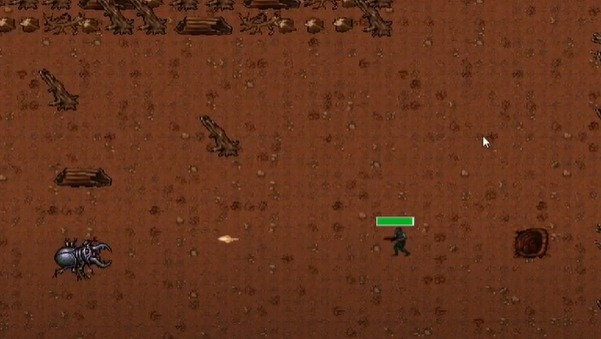
\includegraphics[width=6cm]{Imagenes/pixhell.jpeg}
\centering
\caption{pixHell}
\label{fig:pixhell}
\end{figure}
\section{Objetivos} \label{contenido}
Mis principales objetivos en esta nueva experiencia es aprender a usar más herramientas de la GUI de qt, pero lo que de verdad me llama más la atención es aprender a usar el controlador de versiones (Git) a un nivel bastante avanzado.
\end{document}